\documentclass{article}
\usepackage[utf8]{inputenc}
\usepackage{fullpage}
\usepackage{amssymb}
\usepackage{amsmath}
\usepackage{xcolor}
\usepackage{authblk}

%\title{Multi-parameter optimization and model extrapolation on malaria data}
% ICC: 
\title{Multi-parameter optimization and model extrapolation on/using antimalarial drug screening data}
\author[1]{Oliver Watson}
\author[2]{Isidro Cortés-Ciriano}

%Affiliations
\affil[1]{Evariste Technologies Ltd}
\affil[2]{Centre for Molecular Informatics, Department of Chemistry, University of Cambridge, Lensfield Road, Cambridge, CB2 1EW, United Kingdom.}
%\date{November 2018}

\usepackage{natbib}
\usepackage{graphicx}
\usepackage{hyperref}
\setlength{\parindent}{0pt} 


\begin{document}

% AT: I made a bunch of ' to ` edits
% AT: I added a bunch of Figure before \ref{fig: ...} then stopped in case omission was intentional

\maketitle

\section{Abstract}

We demonstrate the applicability of certain quantitative techniques to address practical problems encountered in small molecule drug discovery.  Specifically we look at using machine learning techniques to predict variables of interest (activity, toxicity) from QSAR inputs, using mathematical and probabilistic arguments in order to build models on biased data (in our case, a dataset that only reports compounds that are active) that will nonetheless generalise to arbitrary datasets, and optimization methods that will maximise the likelihood of obtaining a compound with the desired features.  We use data from ChEMBL malaria assays to obtain values for potency against the malaria parasite \textit{Plasmodium Falciparum} and toxicity against human HepG5 cell lines.  We use data from a commercial vendor (Molport) to examine the predictions our models make on data that is genuinely different from any on which they were fit. Altogether, we believe that this set of techniques represents a self-contained and systematic approach to the problem of selecting compounds for synthesis and testing in a hit-to-lead drug discovery project.
\newpage


\section{Introduction}
\textcolor{red}{THE INTRO NEEDS MORE WORK}
A longstanding goal of artificial intelligence research is to construct algorithms 
to aid in the design of new drugs \cite{Gawehn2016,Chen2018}. 
Whereas deep learning has proved versatile in a number of drug discovery applications\cite{Chen2018}, 
the large number of parameters that need to be optimized often hampers their generalization capabilities. Although multiple algorithms based on neural networks have been proposed to automatize most of the preclinical drug discovery steps, from the generation of structurally novel molecules showing drug-like properties\cite{Kang2018} to the prediction of {\it in vitro} potency and binding affinities\cite{Ozturk2018}, there is still a paucity of integrative and fully data-driven computational pipelines to propose candidate molecules for further experimental testing in an iterative fashion till molecules with the desired properties (e.g., highly potent in an {\it in vitro} biochemical assay and low cytotoxicity) are found.

Here, we present a modelling framework based on a set of multi-parameter optimization algorithms to facilitate automated drug discovery.
We use publicly available data on activity against the most common parasite responsible for malaria: \textit{Plasmodium falciparum}. Our choice was guided by the large amount of data for this particular target that is available in the public domain, and the specific objectives that are associated to a malaria project (for instance, finding drugs that are structurally very different from existing ones).  We discuss in depth two general problems that beset any attempt to use quantitative techniques to direct a drug discovery project: extrapolation and multi-parameter optimization.
% ICC this sounds like a leaflet.. Not good for a publication: In this paper we demonstrate the working of a particular set of algorithms that form part of the proprietary technology developed by some of the authors to facilitate automated drug discovery.  
\newline
\newline


Although we use standard machine learning algorithms in this study, we note that our interpretation of the results is somewhat different from a standard predictive modelling outlook. 
In this work, we formulate and investigate  the tasks of model extrapolation and multi-parameter optimization geometrically, with molecular space $M$ living inside the space $M \to F = [0, 1]^{128}$ associated with 128-bit Morgan fingerprints, and a similarity metric given by Tanimoto distance. 
\newline
\newline
The first question we examine is model extrapolation: given a set of molecules whose values for some feature of interest are known, how well will a model that is trained on this data perform in predicting that same feature for very different molecules? In other words, how well will a model perform when extrapolated away from its training area? This difficulty is particularly acute when trying to build models from public data, due to the biases in the way this data is reported\cite{Kalliokoski2013,Tiikkainen2013}. Here, we show how to use the geometry of molecular space embedded in $F$ to correct for this bias. Our results indicate a way in which predictive models can be trained on a small (and possibly biased) dataset, but notheless produce sensible generalisations when predicting on arbitrary inputs.
\newline
\newline
The second question we address is that of multi-parameter optimization.  A successful drug requires many different properties and being active against the target is only one of these.  It must also be non-toxic, and have the correct chemical properties to allow it to reach the target inside a human body.  We argue that optimizing for these multiple objectives can be facilitated by considering virtual screening as a geometry problem.
This is again due to the geometry of $F$. The correlation between any two random vectors in very close to zero, due to the size of the dimension of the space.  Thus it should be easy for an optimizer, starting from one point, to move in a `good' direction that is orthogonal to several other directions (which is precisely what a multi-parameter optimizer has to do).  Let $B(m, \epsilon) \subset M$ be the set of molecules that are Tanimoto distance less than or equal to $\epsilon$ from the molecule $m$.  The difficulty comes from the fact that given some molecule $m \in M$, the number of molecules in  $B(m, \epsilon)$ may be small for small $\epsilon$, so that although it is easy to find a vector direction starting from a particular molecule in which to search for an improvement, there just aren't any nearby molecules \textit{in that direction}. However, the number of molecules in $B(m, \epsilon)$ grows extremely fast as a function of $\epsilon$.  Our results indicate that correctly adjusted models will generate informative predictions for values of $\epsilon$ sufficiently large that there are in fact plenty of molecules to chose from in any desired direction.



\section{Methods}

\subsection{Collection and Curation of Antimalarial Drug Screening Data}

For this project we gathered antimalarial screening data from ChEMBL database version 23 using the {\it chembl\_webresource\_client} python module\cite{Davies2015}.
Specifically, we assembled a first data set by downloading potency values against \textit{Plasmodium Falciparum} from the following seven Malaria assays available in ChEMBL, namely: GSK TCAMS, St Jude, MMV Malaria Box, Novartis, Harvard, OpenS, and WHO-TDR.
IC50 values were modeled in a logarithmic scale (pIC50 = -log10 IC50 [M]). This data set is available on request (and the code to download directly from Chembl is on the git page accompanying this paper).
\newline
\newline
In addition, we assembled a second data set by downloading antimalarial screening (i.e., potency) and {\it in vitro} toxicity data (50\% growth inhibition bioassay end-point values measured by screesning the compounds in the data set against the cell line HEPG5) from the Tres Cantos data set, downloaded directly from \href{https://chembl.gitbook.io/chembl-ntd/downloads/deposited-set-1-gsk-tcams-dataset-20th-may-2010}{here}. The toxicity values from this data set were used to build the toxicity models described below.
\newline
\newline


It is important to restrict the data one queries from ChEMBL to \textit{specifically} malaria assays performed under controlled experimental conditions, otherwise one obtains a fairly startling variety of results. 
%Earlier on, we attempted to 
For instance, by simply extracting all screening data annotated against 
%run the study on all Chembl values recorded against
\textit{Plasmodium Falciparum} we found over 1,000 different values for Chloroquine activity. What was worse, the standard deviation of the recorded values for Chloroquine was greater than that for the data as a whole. This is line with previous large-scale analysis of the concordance of public data\cite{Kalliokoski2013,Kalliokoski2013B,Cortes-Ciriano2015}, and reinforces the need for stringent filtering and curation steps to gather high quality data prior to modelling.

Using the specific malaria assays gives a much more consistent dataset.  However, we note that the dataset we assembled is biased towards active molecules. It is apparent from the distribution of potency values  that \textit{inactive} molecules are underrepresented (Figure \ref{fig:hist}).  Moreover, we can \textit{not} assume that all other ChEMBL data are inactive against \textit{Plasmodium}, as several well-known drugs (and hence active) are missing from the data. Dealing with this non-trivial bias in the data is a key issue we confront in the model fitting phase (see below).\newline

\begin{figure}[h!]
\centering
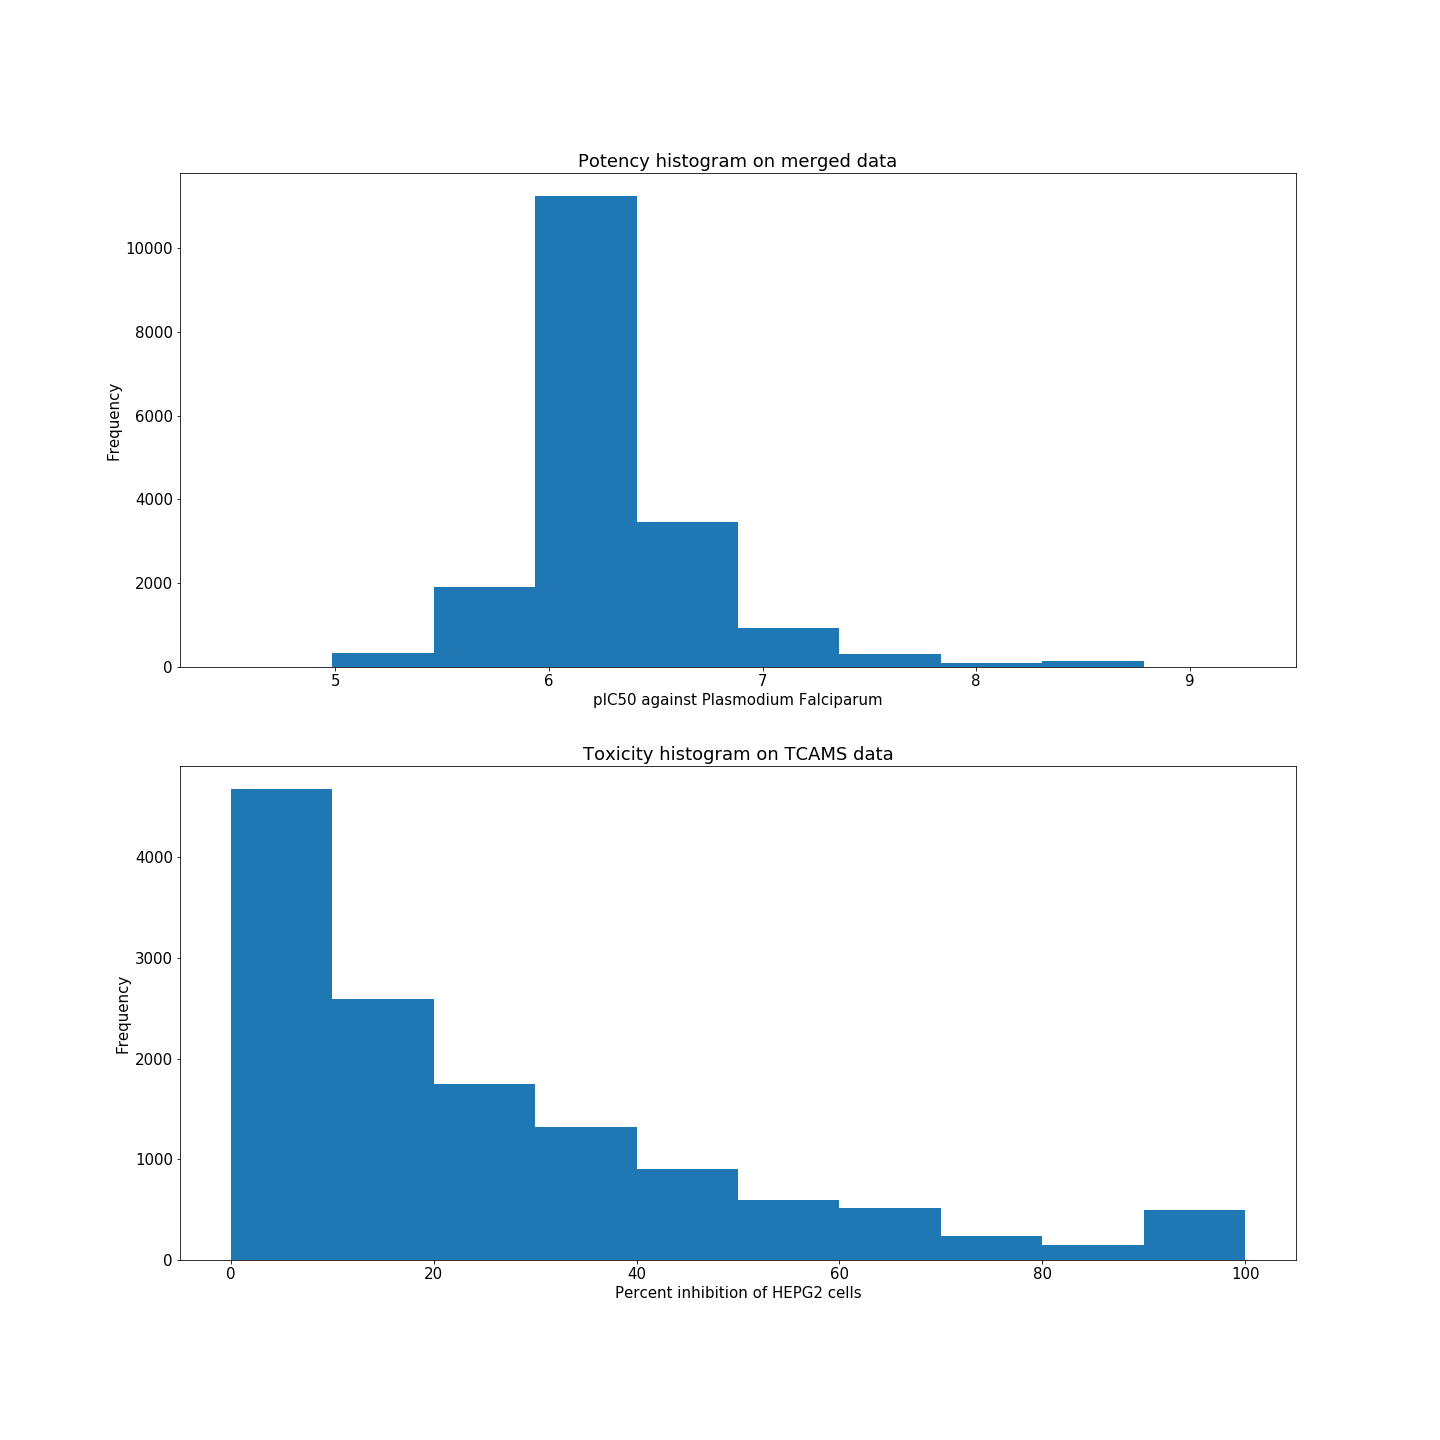
\includegraphics[width=\textwidth]{fig1_hists.png}
\caption{Histograms for toxicity and potency data}
\label{fig:hist}
\end{figure}

\newline
Finally, we used a third data source to explore the commercially available chemical space during the optimization steps.  This is the library of (approximately) 7.5M commercially available compounds from Molport.  We use these compounds as: \begin{itemize}
    \item A proxy for `accessible molecular space'.
    \item A domain from which to select the most promising compounds according to various optimization criteria we investigate (see below).
\end{itemize}


\subsection{Molecular Representation}
We standardized all chemical structures in all datasets described above to a common representation scheme using the python module standardizer (https://github.com/flatkinson/standardiser). Inorganic molecules were removed, and the largest fragment was kept in order to filter out counterions. 
To represent molecules for subsequent model generation, we computed circular Morgan fingerprints\cite{Rogers2010} for all compounds using RDkit (release version 2013.03.02)\cite{rdkit}. We decided to use Morgan fingerprints as compound descriptors given the higher retrieval rates obtained with this descriptor type in comparative virtual screening studies\cite{Koutsoukas2013}. The radius was set to 2 and the fingerprint length to 128. We note that longer fingerprints are associated with higher predictive power. However, we did not observe a large improvement when we used longer fingerprints to model this particular data set. Hence, we decided to use short fingerprints to decrease the computational footprint of our analyses. 

\subsection{Machine Learning}
We built Random Forest (RF) and Ridge Regression models using the python library scikit-learn\cite{scikit}, we previously described \citep{et1:}.
In order to assess the predictive power of the models, we performed K-fold cross validation. Specifically, 
we trained RF and Ridge Regression models on bootstrap subsamples of the data, and used the out-of-sample (OOS) results for each subsample to calculate the RMSE and R2 values for the predicted against the observed potency or toxicity values.
In the vein of generating reproducible research\cite{Walters2013,Landrum2012}, all code used to generate this research, as well as the Jupyter notebook are available at https://github.com/owatson/MalariaPaper (datasets other than Molport data available upon request).




%--------------------------------------
\section{Results and Discussion}
%--------------------------------------

\subsection{Modelling compound potency and toxicity against {\it Plasmodium Falciparum}
%Virtual screening enabled by multiparameter-optimization}
%Geometrical Interpretation of Model Extrapolation and Multi-Parameter Optimization
}

We initially sought to determine the predictive power of RF and Ridge Regression models trained on the full data set.  To estimate these quantities we took 40 random bootstrap samples of our data on which to fit our models (be they ridge regression or random forest) and then used the non-sampled data to compute a value for the quantity (beta, correlation coefficient) of interest.  Confidence intervals were then taken from the resulting distribution of values.

We show below the mean and the 95\% confidence intervals for the Pearson correlation coefficients ($R^2$) between the predicted and observed potency/toxicity values \footnote{We don't show the betas of these models, since these were never statistically significantly different from 1.0 - i.e. these models neither overfit nor underfit}: 

\begin{table}[h!]
\centering
 \begin{tabular}{||c c c c||} 
 \hline
 Result & Mean & Lower 5\% Bound & Upper 5\% Bound \\ [0.5ex] 
 \hline\hline
Potency Ridge Regression $R^2$ & 0.111 & 0.098 & 0.124 \\ 
 \hline
Potency Random Forest $R^2$ & 0.304 & 0.282 & 0.327 \\
 \hline
Toxicity Ridge Regression $R^2$ & 0.125 & 0.106 & 0.139 \\
 \hline
Toxicity Random Forest $R^2$ & 0.299 & 0.287 & 0.309\\
 \hline
\end{tabular}
\caption{Modelling results for Potency and Toxicity using 128-bit fingerprints}
\label{table:Potency}
\end{table}


These results are in accordance with expectation given the results of \citep{et1:} and models reported in the literature for data sets extracted from ChEMBL: Random forests substantially outperform simple linear models when there are no constraints on the in-sample/out-of-sample division.

We also examined the predictive power of models trained using hashed Morgan fingerprints as predictors \footnote{i.e. using the rdkit function GetHashedMorganFingerprint - which returns values in $\mathbb{N}^{128}$ - in particular counting the number of atoms - rather than the simpler GetMorganFingerprintAsBitVect which returns values in ${F_2}^{128}$}  These underperformed (non statistically significantly; Kolmogorov-Smirnov test; P $>$0.05) relative to binary fingerprints in predicting potency, and outperformed (again without statistical significance) in predicting toxicity.  
Given the comparable results of both types of fingerprints, We will only refer to the models based on binary fingerprints for the remainder of the paper.
\newline
\newline

% we obtained metrics on the bootstrap out-of-sample (OOS) fits of both RF and Ridge Regression models we trained the models on bootstrap subsamples of the data, and used the out-of-sample results for each subsample to calculate the OOS metrics. 

%Our basic model fitting procedure was very simple.  For our predictors, we used 128-bit (radius 2) binary fingerprints of the compounds. 

\subsection{Molecular Similarity: Tanimoto distance}

Quantifying molecular similarity is key to chemoinformatic applications in general\cite{Bender2004b}, and to our formulation of virtual screening as a geometry problem in particular.
The standard distance metric used to measure similarity and dissimilarity of molecules is the Tanimoto (sometimes called Jaccard) distance metric\cite{Bajusz2015}.  We wish in this section to develop some intuition for why this metric is the right one for our analysis, and its basic properties.
We map molecules into a binary vector space of some high dimension (128 in this work). In this vector space a `1' implies the existence of some specific molecular substructure in the molecule, and `0' implies its absence.  \newline
\newline
The Tanimoto similarity of two binary fingerprints $A$ and $B$ is simply the ratio of the size of the intersection of $A$ and $B$ over the size of the union of $A$ and $B$\cite{Bajusz2015}. In our setting, it is the number of substructures common to the two compounds represented by $A$ and $B$, divided by the total number of substructures that appear in at least one of the two compounds. The Tanimoto distance is simply 1 - Tanimoto similarity.  The intuitive plausibility for this being a reasonable metric on molecular space is that two compounds that share no features in common should presumably be maximally different (unlike say in the Euclidean metric, where two compounds that each only contained one substructure, different in either case, would be very similar).
\newline
\newline
A good metric in our context will be one for whom it is true that molecules close in that metric have similar toxicity and potency values, and we show in the next section that this is indeed the case for these quantities.
Suppose that any particular substructure has a one-in-two chance of being found in a (randomly chosen somehow) molecule.  The molecular fingerprints would have each bit randomly being 1 or 0 with equal probability $1/2$.  If this were the case, then for two random compounds $A$ and $B$, there would be approximately $1/4$ of the bits both 1 in their fingerprints, and $3/4$ of the bits 1 in at least one of the their fingerprints.  Hence the Tanimoto similarity between $A$ and $B$ would be $1/3$ and the Tanimoto distance would be $2/3$.  More generally, if one could think of molecules as randomly having any given molecular structure with fixed probability $p$, then the Tanimoto distance between two random molecules would be give by $(2-2p)/(2 - p)$.
\newline
\newline
Empirically, looking at the sets of molecules we will be dealing with, the average Tanimoto distance between two randomly selected molecules is around $0.7$, (see Figure \ref{fig:model_extrap}) - showing that a simple model of 'each substructure is present in any compound with probability (slightly under) $1/2$' is not too inaccurate.
\newline
\newline
Given that we are interested in finding potent molecules structurally dissimilar to those in the training data, we next sought to determine the relationship between Tanimoto distance and compound potency (Figure \ref{fig:cov}). Specifically, We collected all pairs of potency values (resp, for molecules $m, n: m \neq n$) and calculated the standard deviation of the potency (resp. toxicity) as a function of the Tanimoto distance $D(m, n)$. This allowed us to quantify the rate of change in these quantities as one moves around in molecular space, or how correlated the potency and toxicity of two compounds will be, depending on how similar they are. We note however that in the case of potency at least, this correlation needs to be adjusted for bias, as we describe in a later section.

\begin{figure}[h!]
\centering
\includegraphics[width=\textwidth]{fig2_same_and_opposite.png}
\caption{Examples of a) same fingerprint, different potency, and b) opposite (Tanimoto distance 1.0) fingerprints}
\label{fig:examples}
\end{figure}


Overall, the fact that the standard deviation increases (and thus correlation decreases) between the potency and toxicity of two compounds as they move further away from each other in Tanimoto distance shows that Tanimoto distance is an appropriate metric to use empirically, as well as theoretically, for this data set.  We will pursue this idea in the next subsections.  


\subsection{Co-variance of Molecular Properties as a Function of Tanimoto Similarity}

Next, we investigated the following question.  Suppose we know some value of interest (say potency, or toxicity) for some compound X.  How much uncertainty is there in our knowledge of that value for some other compound Y, depending on how similar X and Y are?
\newline
\newline
Clearly if Y is very dissimilar to X (essentially a randomly chosen compound) then knowledge of X's properties will tell us nothing about those of Y. Thus our uncertainty about the Y's properties will be the `base rate' uncertainty for those properties. If on the other hand Y is very similar to X, presumably our uncertainty about Y's properties will diminish (this is in some sense the `whole point' of doing any kind of QSAR modelling).  In an extreme case we can imagine that Y is \textit{exactly the same} compound as X - in which case the true uncertainty will be 0 (although the data uncertainty - representing noise in assays or data collection - might be substantially higher than 0).  In this work we use 128-bit binary fingerprints as our mathematical representation of compounds.  Two compounds can have the same 128-bit representation without being identical as we show in figure \ref{fig:examples} (together with an example of two compounds with 'opposite' fingerprints - or ones that are at maximum Tanimoto distance 1.0 from each other.

\begin{figure}[h!]
\centering
\includegraphics[width=\textwidth]{fig3_covariance.jpg}
\caption{Potency and Toxicity Covariance}
\label{fig:cov}
\end{figure}
\newline
Understanding the extent of the uncertainty reduction as as function of the similarity between two compounds is key to one aspect of quantitative drug discovery.  When we select a set of compounds to test, we want to maximize the \textit{information gain} we achieve by testing that set of compounds (subject to minimizing the cost of testing).  Clearly, if the compounds we test are too similar, the information we glean is lower (since knowledge of any one of the test outcomes would tell us a lot about the expected outcome of all the other tests).  This is a principled way to address the question of `Exploration vs. Exploitation'.  We try to test compounds that we expect to be \textit{good}, but also ones that are not too similar to each other.

\subsection{Model Extrapolation as a function of Tanimoto distance}
It is intuitively plausible, and well known among practicing chemists, that models perform poorly on molecules that are \textit{different} form those that the models where trained upon\cite{et0:}.  In this section we attempt to formalize this notion.  We have already seen that that Tanimoto distance provides a plausible and empirically successful measure of distance on molecular space.
\newline
\newline
We expect our models to degrade in their accuracy as we use them to predict on data points far (in Tanimoto distance) from the training set. We can use the training set to assess the extent of this degradation.
\newline
\newline
The first step in fitting our models is to transform the response variables in our data into (approximately) normally distributed values with mean 0. The mean 0 part is particularly important, so that we do not have to worry about whether, when regressing our predictions against our responses, we need to include a constant term.  Thus from our original data set of responses $r_i$ we obtain normed responses $n_i$.
\newline
\newline
The best accuracy we can possibly hope for is given by the `Leave one out' accuracy.  This is calculated as follows.  For any data point, fit a model on all the other data points, predict for the original data point, and add this prediction to your set.  You will then have a set of predictions ${ p_i }_{i = 1}^N$. The `Leave-one-out' accuracy is thus the accuracy of the predictions $p_i$ versus $r_i$.
\newline
\newline
We can extend this concept as follows:  for any datapoint, fit a model on all the other datapoints that are at least distance d from that point.  Again we have a set of predictions ${ p(d)_i }_{i = 1}^N$ and responses $r_i$.  The `Distance d' accuracy is the accuracy of these predictions.  In particular, this method should (with some important caveats that we address in the next section) give a good estimate of the model accuracy when predicting values on a molecule at distance d away from the training set.  If the `intuition' we refer to at the start of this section is correct, then we should see accuracy degrade significantly as we increase d.
\newline
\newline
Let us define $\beta(d)$ by the following equation:

\begin{equation}
    r_{i} = \beta(d) p(d)_{i} + \epsilon
\end{equation}

where $r_{i}$ is some response value of interest, and $p(d)_{i}$ is the prediction obtained from a model (of unspecified type) fit on all datapoints $m_{k} : \mathbf{TD}(m_{k}, r_{i}) > d$
\newline
\newline
Similarly, we can define $R(d)$ as the fraction of the variance  of the $r_{i}$ explained by the equation above  (aka the R-squared of the model).
\newline
\newline
Figures \ref{fig:model_extrap} show plots of $\beta(d)$ and $R(d)$ where the $r_{i}$ is the log potency in the Tres Cantos data set, as a function of $d$.  In each plot we show the functions arising from Random-Forest fits and ridge regression models (both chosen with reasonable parameters, as described in \citep{et1:}).

\begin{figure}[h!]
\centering
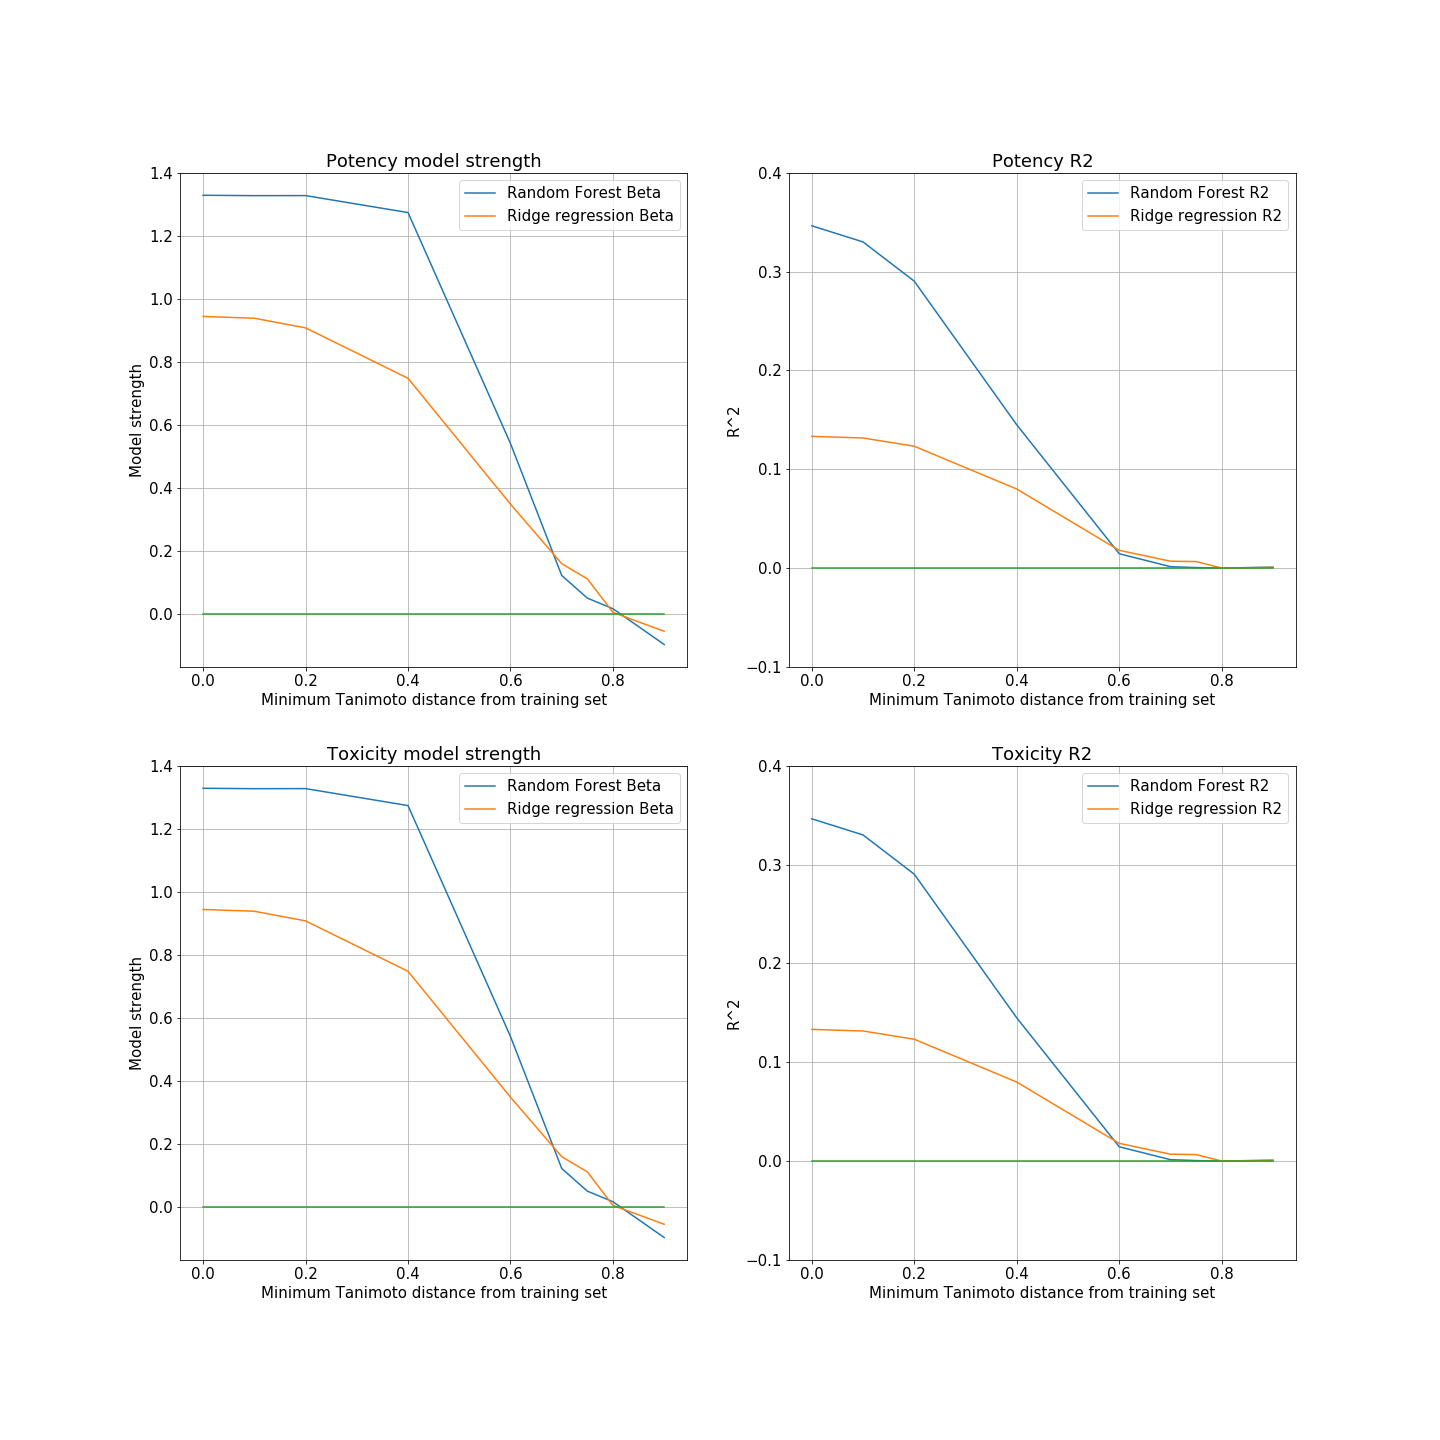
\includegraphics[width=\textwidth, keepaspectratio]{fig4_str_r2.png}
\caption{Model extrapolation as a function of Tanimoto distance}
\label{fig:model_extrap}
\end{figure}


These figures, as one of the main results of this paper, deserve some commentary. First, let us note that in line with general wisdom, the fraction of variance explained by the models decreases as you extrapolate further and further away from the dataset.  Moreover, the Random Forest model dominates the linear model up to extrapolation distance of around 0.6, where in any case, virtually no variance is explained.
\newline
\newline
The results shown relate to earlier work done by the authors in \citep{et0:} and \citep{et1:}.  Note that around extrapolation of Tanimoto distance 0.7, the ridge model still has a small positive beta (i.e. some very small predictive capacity), whereas the Random Forest model now has zero or even negative beta.  This is in line with \citep{et1:} which shows that at sufficient levels of extrapolation, the more constrained linear models outperform the more complex machine learning ones.  However, at this level of extrapolation both models are effectively useless since they explain virtually none of the variance in the data.  
\newline
\newline
What is perhaps most surprising about these results is the quite large extrapolation distance at which the model quality \textit{is not much diminished}.  For example, the Random Forest model at 0.4 extrapolation distance conveys almost half the information as at extrapolation distance 0, where we would have a compound with identical 128-bit fingerprint in our dataset already.

We  employed exactly the same procedure to model toxicity, and found the similar results as shown in the same figure.


\subsection{Correcting for Bias in the Training Data}

Before we can try to apply our models sensibly in a search for potential new drugs, we need to address the issue of the (extreme) bias in the data we have.  Obviously, random compounds are not active against the malaria parasite.  However, it is very clear from looking at a potency histogram of values in our data (Figure \ref{fig:hist}) that (almost) exclusively \textit{active} compounds have been reported.  Nor can we assume that any 'well known' (say present in ChEMBL) compound has been screened against malaria and, if not present in our dataset, is inactive against \textit{Plasmodium Falciparum}.  In particular, some known drugs (Doxycycline) are missing from the data, indicating that we are missing active compounds.

Observing the potency histogram of our malaria data set, we see a peak in pIC50 around $6.5$ (Figure \ref{fig:hist}).  A standard `inactive' molecule would have pIC50 value (to within the limits of experimental error) of less than $4$.  Indeed $3.5$ is the lower limit of many assays, and it is not possible always to measure values below this.  We will assume all \textit{inactive} compounds have a pIC50 of $3.5$ for simplicity.
%ICC I would say a lower limit of 4pIC50 units. And would say that inactives are in the 4-5 pIC50 range normally. We do need to check is these same ranges apply to the assay used to screen the compounds here. One quick way to do that would be to check the pChEMBL values for these compounds
\newline
\newline
We need to make sensible and conservative corrections to our model to allow it to make reasonable predictions on any compound input.  

We do this by breaking the activity prediction into two parts: the activity level (assuming the model is active) and the probability that the compound is active in the first place.  We use a Bayesian calculation, where the conditioning variable is the minimum Tanimoto distance of the compound from any previously seen active (pIC50 > 5) compound.

In Figure \ref{fig:mal_cluster} we show these two density histograms. 
The first one corresponds to 100 million pairwise distances between ten thousand randomly chosen compounds from our malaria dataset.  Thus the first histogram represents the distribution of two compounds that are active against {\it P. falciparum}.

The second density histogram was constructed by calculating another 100 million distances between:
\begin{itemize}
    \item ten thousand randomly selected molecules from the malaria dataset
    \item ten thousand randomly selected molecules from our Molport database.
\end{itemize}
Thus. this histogram represents the distribution of the distance between a molecule active against malaria and a \textit{random} molecule (or at least a random molecule that can be readily obtained in some way).
\newline
\newline
We ask the reader to note two things from this figure:
\begin{enumerate}
    \item Random molecules are quite far (about 0.7) away from each other.
    \item Our malaria data is \textit{not} randomly scattered through molecular space, rather it is (slightly) clustered.  In particular, two molecules in our malaria dataset are much more likely to be close together (even though this probability is still very low) than a random molecule is likely to be near a molecule in our dataset.
\end{enumerate}

We then use these two distributions to estimate the relative density of active vs inactive compounds in the neighborhood of an active compound.

 The key unobserved value that we need to guess at is the fraction of active compounds in the full population of `reasonable' molecules.  
 

 We take it to be $0.01$.  Given that we have just under twenty thousand active compounds, this would indicate that these were obtained from a high throughput screen of around two million compounds, 
which is amenable to current high-throughput technologies\cite{PaweSzymanskiMagdalenaMarkowicz2012}

\begin{figure}
    \centering
    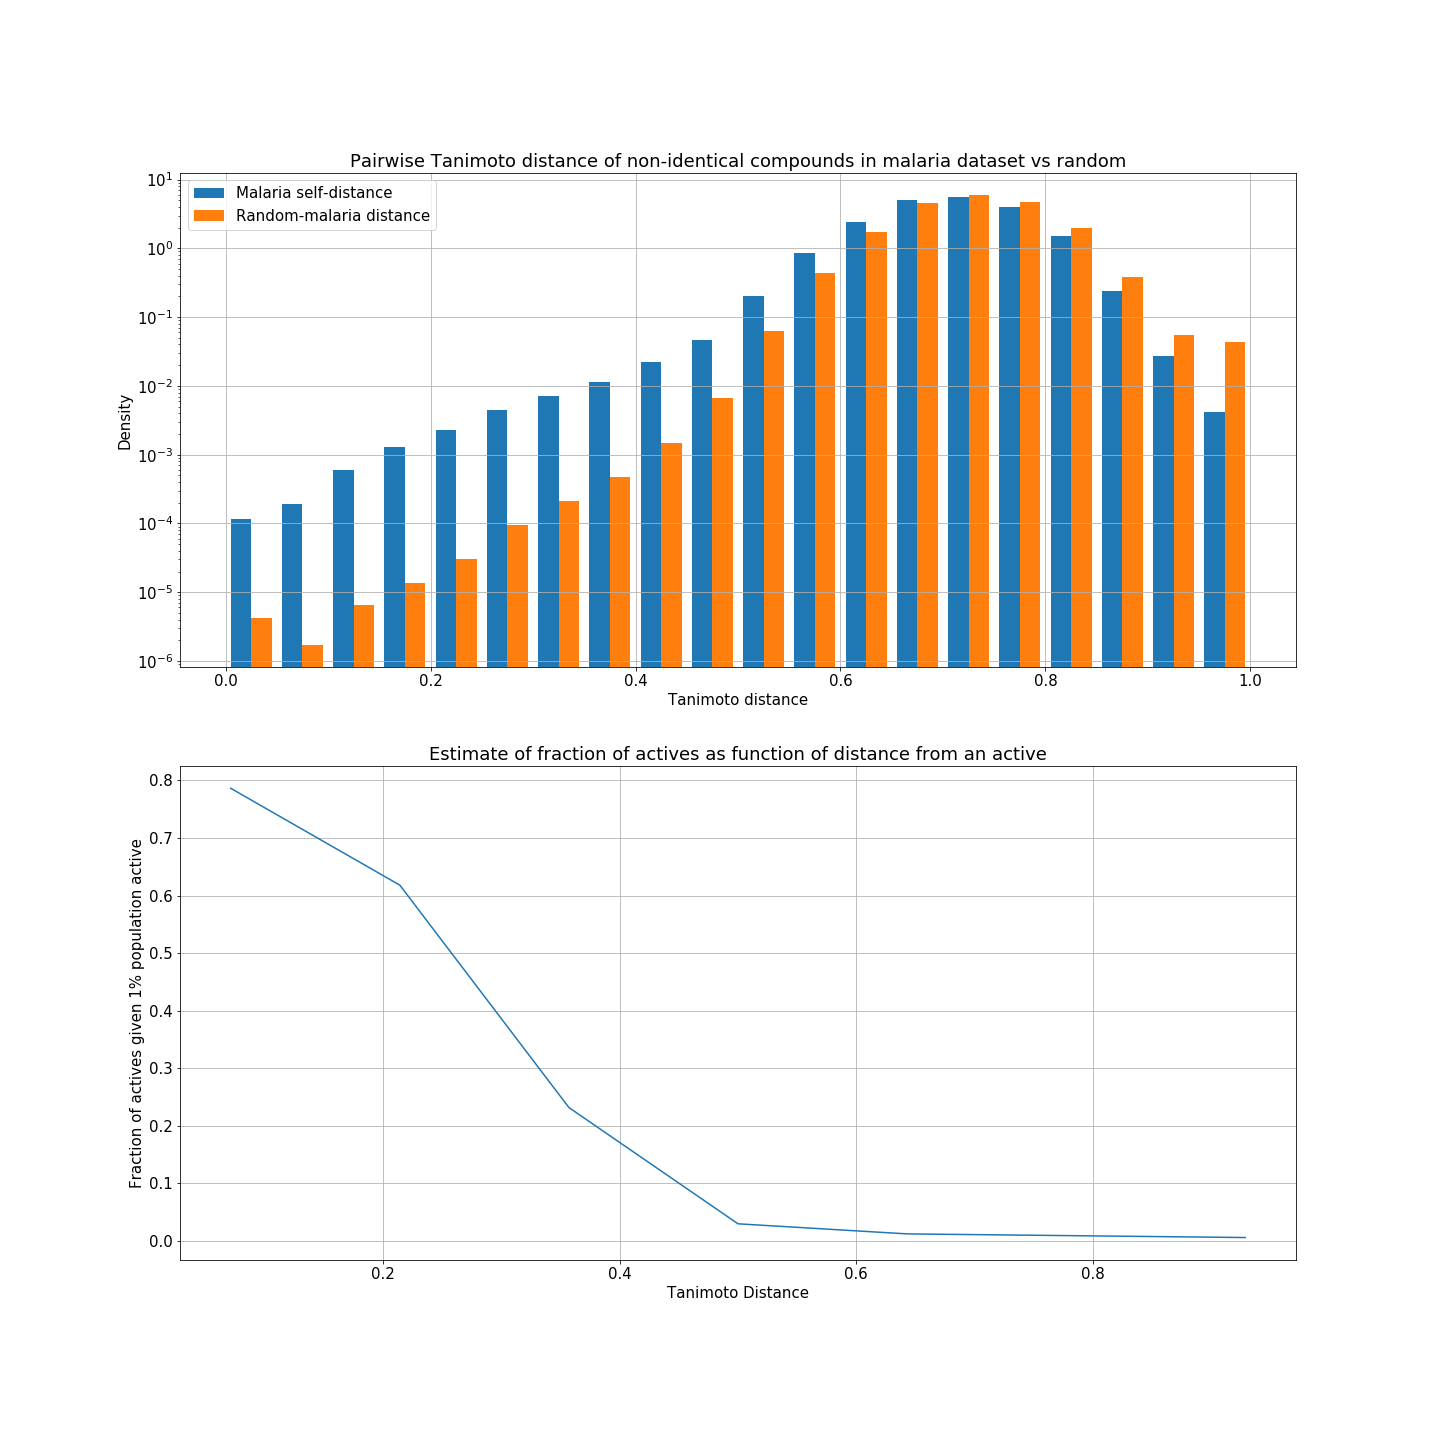
\includegraphics[width=\textwidth]{fig5_bias_correction.png}
    \caption{Bias correction to estimate location of inactives}
    \label{fig:mal_cluster}
\end{figure}

Almost all molecules are inactive, so we can assume the inactive molecules look like random molecules.  Therefore, we can now estimate the density of inactive molecules in the neighborhood of an active one, the key point we need in order to estimate how to generalise our model.  To do this we simply take our estimate of the density between actives (the blue bars in Figure \ref{fig:mal_cluster}) and divide by 100 times the density of the random molecules (recall we assumed there were 100 inactive molecules for every one active molecule).  This gives us an estimate of the probability of being active as a function of the minimum Tanimoto distance from a known active in the lower part of Figure \ref{fig:mal_cluster}.

If we use this plot to estimate the density of actives in the neighborhood of another active, this model will be conservative in the following sense.  It will \textit{underestimate} the fraction of actives in some neighborhood of an active; the true density will lie above our estimated density in the neighborhood of 0 (and look more like a cliff than a gradual decline).  In practice, this will mean that a model incorporating this estimate of the distribution of inactives will, when used to select the most promising new compounds for testing, select ones slightly closer to known active molecules than in optimal. We do not attempt to correct for this bias, but believe it to be worth noting. The reason the model is biased this way is the following. When we estimate the location of the inactives, we only take into account the clustering of the malaria data in molecular space, filling in the `gaps' uniformly with inactive compounds.  However, as Figure \ref{fig:cov} shows, two nearby active molecules are more likely to have similar activity levels than two more distant ones; covariance in activity for the \textit{active} molecules increases as a function of distance in Tanimoto space.  Surely therefore if there is less uncertainty in the activity level of an active molecule in the close neighborhood of some known active compound C, surely also a general molecule \textit{is more likely to be active} if it lies in the close neighborhood of some known active compound, beyond the simple geometric argument we have given. \footnote{Indeed, we attempted to use the results from Figure \ref{fig:cov} to estimate the density of inactives in the range of an active directly via a Bayesian argument, but the results were unsatisfactory.  If one assumes normally distributed activity levels (or rather half normal, since they can't go below the inactive level) then one gets an implausibly small prior probability of being active.  Given there was no other `natural' choice of variance model to impose on the data, we abandoned this approach in favor of the geometric argument given above.}
\newline
\newline

Thus, at this stage we can finally write down our model in full generality.

For an unknown compound $C$, the predicted potency will be:

\begin{equation}
    \mathbb{E}[Potency(C)] = \mathbb{E}[Potency(C | C \in A)] * \Pr(C \in A) + I * (1-\Pr(C \in A))   
\end{equation}

where $A$ = set of Active molecules and $I$ = activity level of inactive molecules.

In this case $\mathbb{E}[Potency(C | C \in A)]$ will be a function of: \begin{itemize}
    \item our actively fit model prediction on C
    \item the minimum distance of C from our dataset (as C moves further away from our training set in Tanimoto space, we should - from Figure \ref{fig:model_extrap} belief our estimate towards the mean activity level.
\end{itemize}

$\Pr(C \in A)$ is simply a function of the minimum Tanimoto distance of $C$ to the malaria dataset.


With the toxicity data, the nature of the bias (if any) is not as clear.  Therefore, we will not attempt to correct for bias in the toxicity model, and simply take the predictions as they are provided by the model (in particular, we will not belief toxicity prediction towards the mean toxicity as we move further away from the malaria dataset.


% Define MOP
% Reads multi-parameter optimization optimization 
\section{Multi-Parameter Optimization (MPO)}

In this section, we illustrate how the models described above could be used in a drug discovery project. In particular, we illustrate what the models do, and how different goals can be traded off against each other.

We have our models fit on the combined malaria data, but to arrive at new predictions, we need to apply these models to new compounds.  We use the 7.5M commercially available molecules from Molport (Methods), and look at the top selections from these according to our models along various criteria.

As a starting point, what are the compounds predicted to be most potent in the Molport database (removing stereoisomers, or any compounds that have identical 
%rdkit.Chem 
smiles)?  We show the top five in Figure \ref{fig:mostpot}.

\begin{figure}[h!]
\centering
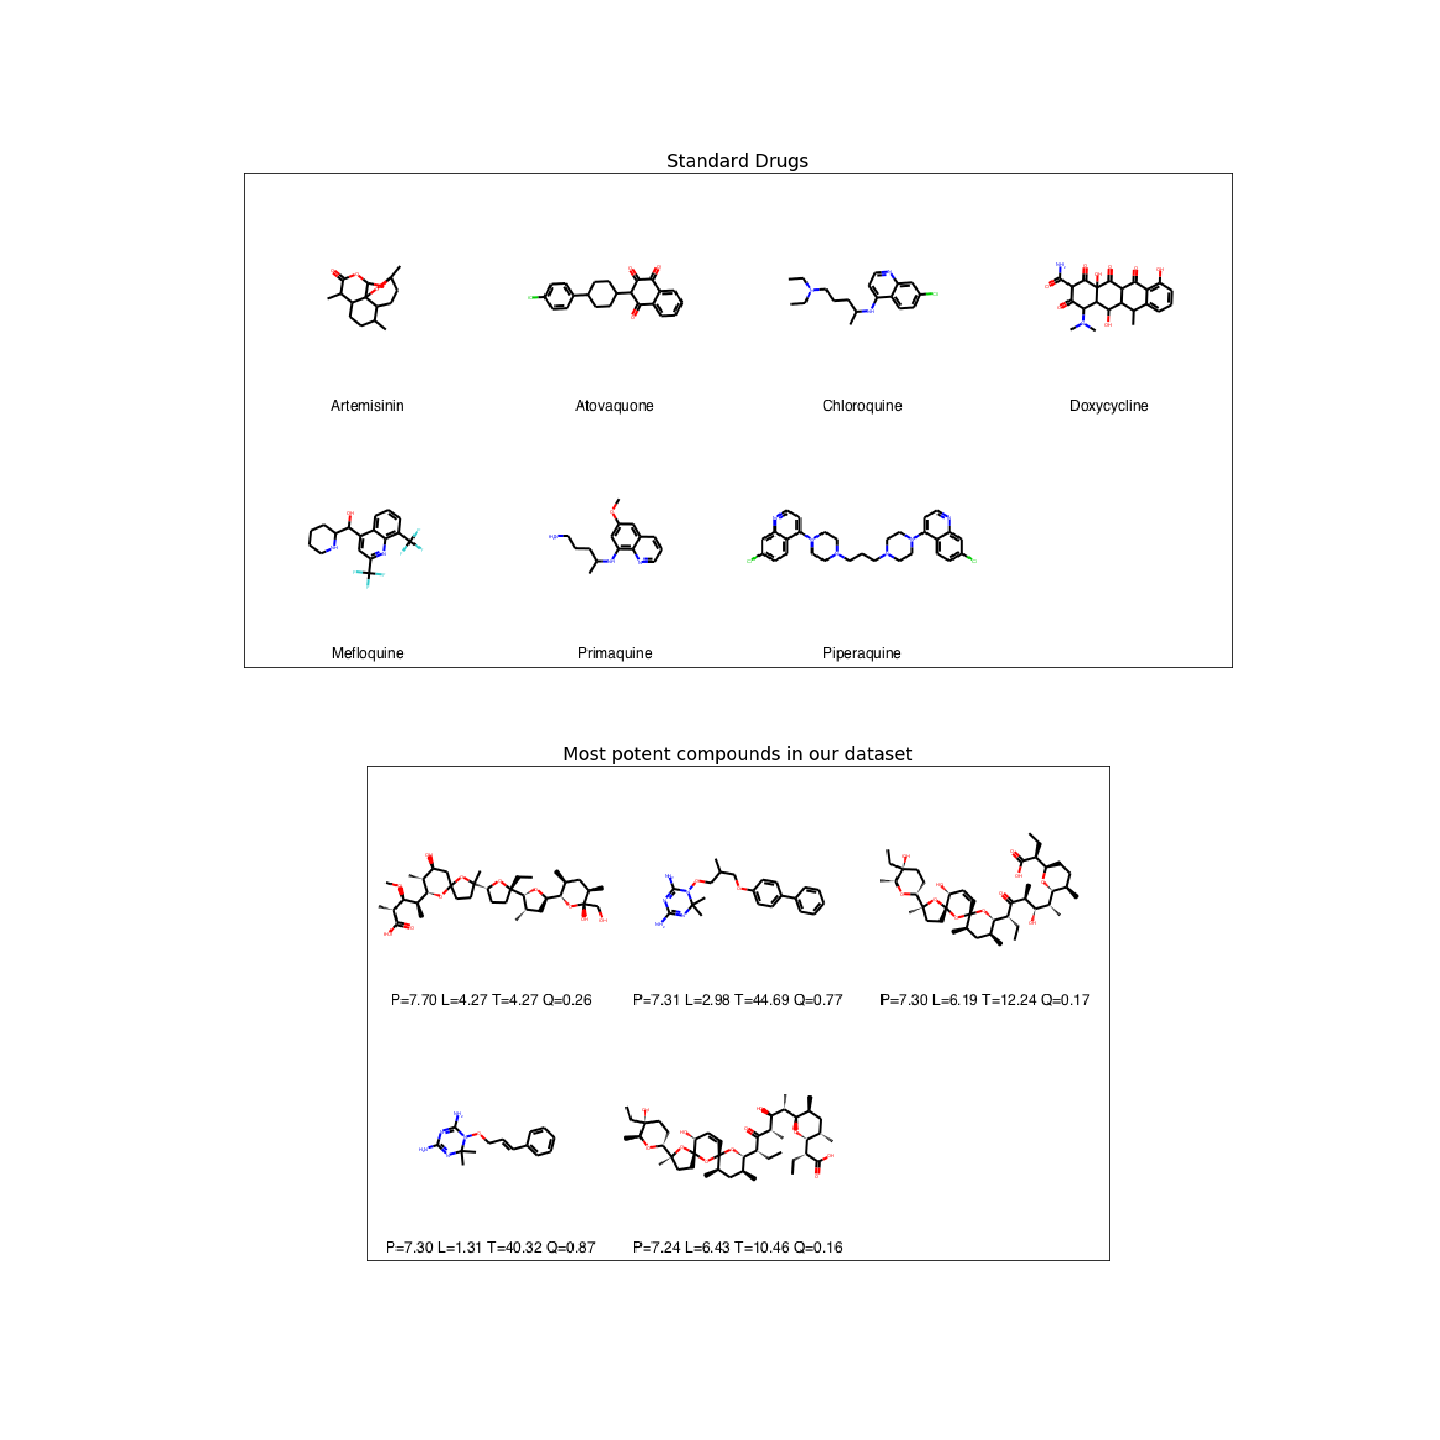
\includegraphics[width=\textwidth]{fig6_drugs_n_pot.png}
\caption{Standard drugs, and our most Potent predicted compounds: P=Potency, L=Lipophilicity, T=Toxicity(\%) Q=QED}
\label{fig:mostpot}
\end{figure}


%This is a fairly uninteresting result.  
All these compounds are (very slight variations on) compounds in our original malaria dataset (all have Tanimoto distance 0 to compounds in the original dataset apart from the fourth compound, which has distance 0.078).  

In particular, note that the logP values of these compounds are not in the range [2-4] (generally thought to be a good indicator of favorable ADMET properties), and QED values are below 0.5 (another ADMET indicator), showing that these compounds may not in fact be particularly suitable for drugs.  The top hit in fact is Monensin, an antibiotic that is known to have anti-malarial activity (see: https://en.wikipedia.org/wiki/Monensin).

If one requires good Lipophilicity and QED values, and low predicted toxicity values, one gets as top suggestions the compounds shown in Figure \ref{fig:best_q}.


\begin{figure}[h!]
\centering
\includegraphics[width=\textwidth]{fig7.png}
\caption{Best Potency, with Lipophilicity and QED thresholds, as well as good Toxicity}
\label{fig:best_q}
\end{figure}


A key goal of drug research in malaria is to develop new drugs, as the parasites evolve immunity to existing ones.  Commercially, one may also want to develop drugs that have different side-effect profiles, or cover novel Intellectual Property space.  We still of course want drugs that are potent, non-toxic, and have favorable ADMET qualities.  For the purposes of a drug discovery program, we want to search as large an area of molecular space as possible, as cheaply as possible.  We distill these qualitative goals into the following list of quantitative requirements. 

\begin{enumerate}
    \item To represent our goal of finding \textit{new} drugs, we take seven of the best-known malaria drugs and require that our selected compounds are at least 0.6 in Tanimoto distance away from any of these.
    \item As an indication of reasonable ADMET properties, we require logP of our compounds to be within the range [2-4]\cite{Hansch1971}.
    \item As an additional indictator of favorable ADMET, we require that QED of the compounds be $> 0.5$.
    \item Predicted toxicity from the Tox models must be $< 25\%$.
\end{enumerate}

This set of requirements picks up a subset of the compounds from our original malaria set, shown in Figure \ref{fig:best_in_data}.  These compounds therefore seem promising starting points for drug discovery programs. To the authors' knowledge these are not in fact actual anti-malarial drugs, although they satisfy all the criteria that we could think of imposing.


\begin{figure}[h!]
\centering
\includegraphics[width=\textwidth]{fig7.png}
\caption{Most potent choices subject to all criteria}
\label{fig:best_in_data}
\end{figure}


It is of course not surprising that we find compounds in our original training set when we look for `most potent' compounds, even with all the other criteria we impose.  The predicted potency given by our model should decrease as we wander further away from the dataset on which it was trained.  Taken together,  these results show that it is possible to satisfy a multi-objective optimization and still find  potent candidates, at least when one has a training set as large as the one we had in this instance.
\newline
\newline
For the purposes of this paper however we want to look at the predictions of the model on compounds that are different from any it has seen before.  Therefore we show in Figure \ref{fig:best_choices} our top selections according to the above criteria \textit{that are also at least 0.2 Tanimoto distant from any molecule in the original malaria dataset}.  We also show in \ref{fig:best_choices_neigbours} the closest compounds in our original dataset to these choices.



The key points to draw from Figure \ref{fig:best_choices} is that a) the potency predictions are reasonable (obviously at the low end of the range of active compounds, since we are deliberately moving away from the training set), b) that given this, we can make sensible probabilistic estimates not only for each compound having potency beyond a certain threshold, but also by using the covariance models in Figure \ref{fig:cov} and \ref{fig:cov}, for \textit{at least one of} our chosen compounds being in a desired range.   We can then use standard optimization techniques (such as simulated annealing) to choose an optimal set of compounds for testing, and can even incorporate information as to the cost of purchasing an testing the compounds into this optimization.  It seems worth mentioning also that although $0.2$ Tanimoto distance is `quite close', and certainly within the range at which our models are expected to predict very well, even at this short distance we are finding compounds that are structurally different from their nearest neighbours in the original malaria dataset.  


%-----------------------------------
\section{Conclusions}
%-----------------------------------
The goal of this paper
%, in addition to presenting some interesting modelling results relating to malaria, 
has been to present a sketch of an alternative modelling framework to pursue quantitative drug discovery.
%how quantitative drug discovery might be pursued.  
In particular, we have shown that models can be fit on molecular data that give reasonably results when applied to \textit{any} molecular inputs, as shown by the fact that when, presented with the full set of commercially available molecules, the models pick up ones they have seen in the training set, but also predict plausible values outside it.  This is important, since unless one has confidence in one's models' predictions for arbitrary inputs, one is forced in optimization to drastically restrict the range in which one searches for a solution.   The fact that we have plausible real-value predictions (i.e., predictions that we expect to neither overestimate nor underestimate the value of interest) and can build proper variance models to accompany them means that we can properly specify an objective function to use in searching over molecular candidates, and achieve direct feedback from experimental results.  In practice, after searching through commercially available compounds, one would couple these algorithms with molecular exploration software\cite{Firth2015,Merk2018}, 
%such as MOARF [insert reference], 
to create an automated drug discovery package.  We plan to describe this process of optimization in a later paper.


%-----------------------------------
\newpage
\section{Author Contributions}
O.W. conceived and designed the study. 
O.W., I.C.C. and J.W. interpreted and analyzed the results, and wrote the paper.

\section{Acknowledgements}
This project has received funding from the European Union’s Framework Programme For Research and Innovation Horizon 2020 (2014-2020) under the Marie Curie Sklodowska-Curie Grant Agreement No. 703543 (I.C.C.).
We would like to thank Molport for making their proprietary screening library available to us for our research.

\section{Conflicts of interest}
O.W. and I.C.C. hold equity interest in Evariste Technologies Ltd.

\newpage

\bibliographystyle{plain}
\bibliography{references}
\end{document}
